\documentclass[a4paper,12pt]{report}

\usepackage[utf8]{inputenc}
\usepackage[T1]{fontenc}
\usepackage[french]{babel} % If you write in French
\usepackage{xcolor,graphicx}


\usepackage{geometry}
\geometry{left=2cm, right=2cm, top=4cm, bottom=4cm}
\usepackage{titlesec}
\usepackage{lmodern}
\usepackage{array}


\usepackage[hidelinks]{hyperref} % Permet de rendre les liens cliquables sans les entourer d'un cadre coloré


\usepackage{fancyhdr} % Pour personnaliser les en-têtes et pieds de page
% Configuration des en-têtes et pieds de page
\pagestyle{fancy}
\fancyhf{} % Efface les en-têtes et pieds de page par défaut
\fancyhead[L]{\leftmark} % Affiche le nom du chapitre à gauche
\fancyfoot[R]{\thepage} % Affiche le numéro de page au centre du pied de page


\usepackage{enumitem}
% Uniquement le premier niveau
\setlist[itemize,1]{label={.}}
% Deuxième niveau avec un point gras
\setlist[itemize,2]{label={\boldmath$\cdot$}}



\usepackage{longtable} % Pour permettre aux tableaux de se répartir sur plusieurs pages


\renewcommand{\arraystretch}{1.5} % Espacement entre les lignes du tableau


\usepackage{booktabs} % Pour un meilleur rendu du tableau
\usepackage{float}



\usepackage{xcolor}
\usepackage{tcolorbox}
\usepackage{listings}

% Définition d'un style de terminal
\newtcbox{\terminalbox}{on line, colback=black, colframe=black, boxrule=0pt, left=3pt, right=3pt, top=2pt, bottom=2pt, boxsep=3pt, sharp corners, enhanced}

\begin{document}



%-------------------------------------------------------------------+
  
\begin{titlepage}
	%  \pagecolor{blue!10}
	\begin{center}
		\begin{minipage}{1.5cm}
			\begin{center}
				
\includegraphics[width=2.5cm,height=1.7cm]{images/logo/logo-arcop.png}

			\end{center}
		\end{minipage}\hfill
		\begin{minipage}{12cm}
			\begin{center}
				\textbf{ Institut de Formation Aux Normes et Technologies de l'Informatique}\\[0.1cm]
				\textbf{-Sokodé-}
				% 		\textsc{\uppercase{Université Sultan Moulay Slimane}}

				% 		\uppercase{éCOLE NATIONALE DES SCIENCES APPLIQUéES KHOURIBGA}
			\end{center}
		\end{minipage}\hfill
		\begin{minipage}{1.5cm}
			\begin{center}
				
\includegraphics[width=2.3cm,height=2.5cm]{images/logo/logo-ifnti.png}
			\end{center}

		\end{minipage}
	
		\textsc{\Large }\\[1cm]
		{\large \bfseries Rapport De Stage de Fin d'\uppercase{é}tudes}\\[0.5cm]
		{\large En vue de l'obtention du diplôme}\\[0.5cm]

		{\huge \bfseries \uppercase{Licence Informatique} \\[0.5cm] }
		{\large \bfseries Filière : Génie Informatique}
		\textsc{\Large }\\[1cm]

		% Title
		\rule{\linewidth}{0.3mm} \\[0.4cm]
		{ \huge \bfseries\color{blue!70!black} Développement et personnalisation d’une solution digitale pour le service des \ac{RH} de l’\ac{ARCOP} \\[0.4cm] }
		\rule{\linewidth}{0.3mm} \\[1cm]

		{\large \bfseries Effectué à : l'\ac{ARCOP} du  15 Aoùt 2024 au 19 Février 2025 }\\[1cm]
		% \includegraphics[width=0.3\textwidth]{logo-isae-supaero}\\[1cm]
		% Author and supervisor
		\noindent
		\begin{minipage}{0.4\textwidth}
			\begin{flushleft} \large
				\emph{\color{orange!80!black}Réalisé par :}\\
				M.~\textsc{AMONA} Birewa Audrey \\
			\end{flushleft}
		\end{minipage}%
		\begin{minipage}{0.5\textwidth}
			\begin{flushright} \large
				\emph{\color{orange!80!black}Encadré par:} \\
				
				M. \textsc{GBOLOVI} Komi Dodzi (\ac{ARCOP})\\
			\end{flushright}
		\end{minipage}\\[1cm]

	

		% \vfill

		% Bottom of the page
		{\large \color{orange!80!black}{Année universitaire}\\ \color{blue!80!black}2023/2024}

	\end{center}
\end{titlepage}

%-------------------------------------------------------------------+
\pagenumbering{Roman}
%-------------------------------------------------------------------+

\chapter*{Remerciements}
%\addcontentsline{toc}{chapter}{Remerciements}
\thispagestyle{empty}

Tout d’abord, je rends grâce à Dieu le Tout-Puissant pour m’avoir accordé la force, le courage et la patience nécessaires à l’accomplissement de ce travail.\\

Je tiens à exprimer ma profonde gratitude à \textbf{M. GBOLOVI Komi Dodzi}, mon tuteur de stage, pour son accompagnement inestimable, la qualité de son suivi ainsi que les conseils et informations qu’il m’a prodigués avec professionnalisme et bienveillance.\\

Mes sincères remerciements vont également à \textbf{M. Aftar Touré MOROU}, Directeur général par intérim de l’Autorité de Régulation de la Commande Publique (\ac{ARCOP}), pour m’avoir offert l’opportunité d’intégrer son équipe et pour son soutien tout au long de cette expérience.\\

Je tiens à exprimer une reconnaissance toute particulière à \textbf{M. TEOURI Sabirou}, dont l’aide précieuse m’a permis d’obtenir ce stage au sein de l’\ac{ARCOP}.\\

J’adresse également mes vifs remerciements à \textbf{M. AFOH TCHAOUTA Charif, Mme Fati Kpandjapou DATAGNI, M. Kouassi HOUESSOU, M. Sinam Hippolyte TOKI}, ainsi qu’à l’ensemble du personnel de la \textbf{Direction des Statistiques et de la Documentation} pour leur accueil chaleureux, leur aide précieuse et leurs encouragements qui ont contribué à rendre mon stage des plus enrichissants.\\

Un grand merci à \textbf{M. GBADJAVI Combété}, Chef de division des ressources humaines et services généraux, pour ses conseils avisés et le soutien qu’il m’a apporté.\\

Je souhaite également exprimer ma gratitude aux membres du jury pour l’honneur qu’ils me font en prenant le temps d’évaluer mon travail.\\

Enfin, je remercie chaleureusement toute l’équipe pédagogique et administrative de l’\textbf{\ac{IFNTI}} pour les efforts qu’elle déploie afin de nous offrir une formation de qualité.\\

À toutes les personnes qui, de près ou de loin, ont contribué à la réalisation de ce travail, je témoigne ici ma reconnaissance infinie.


\clearpage
%-------------------------------------------------------------------+
\chapter*{Résumé}
\addcontentsline{toc}{chapter}{Résumé}
\thispagestyle{empty}
\clearpage
%-------------------------------------------------------------------+

\tableofcontents
\thispagestyle{empty}
\clearpage

\listoffigures
\thispagestyle{empty}
\clearpage

\listoftables
\thispagestyle{empty}
\clearpage

%-------------------------------------------------------------------+
\pagenumbering{arabic}

\chapter{Introduction Générale}
\clearpage
\section{contexte}
Dans le cadre de leur formation, les étudiants en troisième année de l'Institut de Formation aux Normes et Technologies de l'Informatique doivent effectuer un stage de fin d’études au sein d’une organisation avant l’obtention de leur diplôme. Cette immersion professionnelle vise à leur permettre d’acquérir des compétences pratiques et à mieux appréhender le fonctionnement du monde du travail.\\

C’est dans cette perspective que le stage a été réalisé au sein de l’Autorité de Régulation de la Commande Publique (ARCOP). Cette institution joue un rôle central dans la gestion et la régulation des marchés publics, veillant à leur transparence et à leur efficacité. En 2023, l’ARCOP a marqué une avancée significative avec l’application d’une nouvelle réglementation relative aux marchés publics, la formation de plus de 1600 acteurs du secteur, ainsi que l’initiation de plusieurs projets de digitalisation et d’amélioration des procédures.\\

Le présent rapport a pour objectif de présenter les différentes missions effectuées au sein de l’ARCOP, ainsi que les réalisations techniques développées au cours du stage. Il met en lumière les compétences acquises et les défis rencontrés, tout en illustrant l’apport de cette expérience dans le cadre de la formation académique.\\

\section{Objectifs}
L’objectif principal de ce stage de fin d’études est de permettre à l’étudiant de mettre en pratique ce qu’il aura acquis tout au long de sa formation en licence d’informatique des organisations à l’IFNTI, que ce soit en termes de compétences techniques comme de compétences humaines et professionnelles. L’étudiant devra être capable de s’adapter rapidement aux besoins de l’organisation afin de s’intégrer aux projets sur lesquels il travaillera. La prise en compte des démarches qualités et des méthodes associées au sein de l’organisation est primordiale. Enfin, ce stage doit permettre à l’étudiant d’acquérir une certaine autonomie technique.\\
Tout au long du stage, l’étudiant doit être accompagné d’un maitre de stage ayant entre autres pour role de l’accompagner dans son intégration au fonctionnement de l’organisation, mais aussi de le suivre en se rendant disponible.
%-------------------------------------------------------------------+
\chapter{Présentation de l'organisme d'acceuil}
\clearpage
\section{Historique et missions de l’ARCOP}

\subsection{Historique}
En vue de l’instauration d’un État de droit prospère, le gouvernement togolais a entrepris de profondes réformes institutionnelles. Ainsi, pour se conformer aux dispositions régionales, il a été mis en place l’Autorité de régulation de la commande publique (ARCOP), une autorité administrative indépendante investie de plusieurs missions selon les dispositions du décret n° 2009-296/PR du 30 décembre 2009, modifié par le décret n° 2011-182/PR du 28 décembre 2011 portant missions, attributions, organisation et fonctionnement de l’Autorité de Régulation de la Commande Publique.

L’Autorité de régulation de la commande publique est située sur le boulevard GNASSINGBE Eyadema. Elle est logée aux 6ème et 7ème étages de l’immeuble SANLAM, près du siège de Yas-TOGO.

\begin{itemize}
    \item \textbf{Adresse :} B.P. 12 484 Lomé-Togo
    \item \textbf{Téléphone :} (00228) 22 23 06 80 / 22 23 06 81
    \item \textbf{E-mail :} \href{arcoptogo@arcop.tg}{arcoptogo@arcop.tg}
    \item \textbf{Site web :} \href{https://arcop.tg}{https://arcop.tg}
    \item \textbf{N° vert :} 80 00 88 88
\end{itemize}

\subsection{Missions de l’ARCOP}
Selon l’article n° 3 du décret n° 2022-063/PR, \og l’Autorité de régulation de la commande publique assure la régulation du système de gestion de la commande publique \fg.

À ce titre, elle :
\begin{itemize}
    \item Émet des avis, propositions ou recommandations dans le cadre de la définition des politiques et de l'assistance à l'élaboration de la réglementation de la commande publique ;
    \item Assure la sensibilisation et l'information des acteurs de la commande publique ;
    \item Élabore des stratégies de professionnalisation et de renforcement des capacités ;
    \item Assure l’évaluation des performances du système de passation et d’exécution ;
    \item Diligente des enquêtes sur les irrégularités et violations ;
    \item Initie des procédures d'audits de conformité et financiers ;
    \item Procède au règlement non juridictionnel des litiges et sanctionne les irrégularités constatées.
\end{itemize}

\section{Les organes de l’ARCOP}
Conformément aux dispositions du décret n° 2009-296/PR modifié, l’ARCOP est composée de trois organes :
\begin{itemize}
    \item Le Conseil de régulation (CR) ;
    \item Le Comité de règlement des différends (CRD) ;
    \item La Direction générale (DG).
\end{itemize}

\subsection{Le Conseil de régulation (CR)}
L’article n° 11 du décret n° 2022-063/PR stipule que le conseil de régulation est un organe tripartite composé de neuf membres représentant l’administration publique, le secteur privé et la société civile.

\subsection{Le Comité de règlement des différends (CRD)}
L’article n° 22 du décret n° 2022-063/PR stipule que le comité de règlement des différends est chargé de :
\begin{itemize}
    \item Examiner les recours relatifs à la passation des contrats de la commande publique ;
    \item Statuer sur les irrégularités ou violations constatées ;
    \item Régler les différends entre entités administratives impliquées dans la commande publique.
\end{itemize}

\subsection{La Direction générale}
L’article n° 29 du décret n° 2022-063/PR stipule que la direction générale est l'organe exécutif de l’ARCOP, chargée de l’application des politiques générales et de la mise en œuvre des décisions du conseil de régulation.

Elle est structurée en six directions :
\begin{itemize}
    \item \textbf{Direction des services administratifs et financiers (DSAF)} : gestion des ressources humaines et financières ;
    \item \textbf{Direction de la réglementation et des affaires juridiques (DRAJ)} : suivi et mise en application des réglementations ;
    \item \textbf{Direction de la formation et des appuis techniques (DFAT)} : renforcement des capacités des acteurs ;
    \item \textbf{Direction des statistiques, documentation et suivi-évaluation (DSD-SE)} : centralisation des données et évaluation des performances ;
    \item \textbf{Direction des investigations et enquêtes (DIE)} : enquêtes sur les irrégularités et lutte contre la corruption ;
    \item \textbf{Direction de la communication et des relations publiques (DCRP)} : gestion de la communication interne et externe.
\end{itemize}

La Direction générale de l’ARCOP exerce une surveillance active sur les processus d'achat public afin de garantir l'intégrité, la transparence et l'efficacité des dépenses publiques, contribuant ainsi au développement économique et social du pays.



\clearpage
%-------------------------------------------------------------------+
\chapter{Déroulement factuel du stage}
\clearpage

\section{ Prise de fonction et intégration}
À mon arrivée à l’ARCOP, j’ai été accueilli au sein de la Direction des Statistiques et de la Documentation. Après une présentation de l’organisation et des missions du service, j’ai pris connaissance des objectifs du stage ainsi que des attentes de mon tuteur.

Durant cette phase d’intégration, j’ai également :
\begin{itemize}
    \item Découvert l’environnement de travail et les outils utilisés.
    \item Pris en main les méthodologies internes et les processus en place.
    \item Échangé avec les membres de l’équipe pour mieux comprendre les besoins et le cadre du stage.

\end{itemize}
\section{Découverte du projet principal et études préliminaires}
L’objectif principal de mon stage était la \textbf{digitalisation des processus de travail du département des ressources humaines (RH)}. Avant d’entamer le développement, plusieurs tâches préparatoires ont été réalisées :




\begin{itemize}
    \item Analyse des besoins du département en collaboration avec le responsable RH.
    \item Étude des solutions existantes et identification des axes d’amélioration.
    \item Participation aux réunions pour recueillir les attentes des utilisateurs.
    \item Rédaction d’un cahier des charges et validation des fonctionnalités essentielles avec mon tuteur.
\end{itemize}

\section{Développement de la solution numérique}
Après cette phase d’étude, j’ai entamé la conception et le développement de l’application. Cela a inclus :
\begin{itemize}
    \item La mise en place de l’environnement de développement (choix des technologies, configuration des outils).
    \item La conception de l’architecture du projet et de la base de données.
    \item Le développement des premières fonctionnalités, notamment \textbf{ l’authentification et la gestion des utilisateurs}.
    \item Des tests et des ajustements basés sur les retours du tuteur et des futurs utilisateurs.

\end{itemize}
Par la suite, d’autres fonctionnalités ont été intégrées, comme :

\begin{itemize}
    \item La gestion des documents administratifs.
    \item L’automatisation de certaines tâches RH.
    \item L’amélioration de l’interface utilisateur pour une meilleure expérience.
\end{itemize}


\section{Participation au service de support et aux tâches techniques}
En parallèle du développement de mon projet principal, j’ai apporté mon aide à plusieurs niveaux du support technique, notamment :
\begin{itemize}
    \item \textbf{Support aux utilisateurs de la plateforme PASSE :} 
    \begin{itemize}
        \item Réponse aux demandes des utilisateurs rencontrant des difficultés techniques.
        \item Diagnostic et résolution des bugs signalés.
    \end{itemize}
    \item \textbf{Installation et maintenance des équipements informatiques :} \begin{itemize}
        \item Installation et configuration d’ordinateurs de bureau pour les employés.
        \item Installation et mise à jour d’antivirus pour renforcer la sécurité informatique.
    \end{itemize}
    \item \textbf{Débogage du réseau téléphonique IP de l’entreprise :} \begin{itemize}
        \item Analyse des dysfonctionnements et recherche des causes des interruptions de service.
        \item Participation aux interventions techniques pour rétablir la connexion et améliorer la qualité des appels.
    \end{itemize}
\end{itemize}

Cette expérience m’a offert une meilleure compréhension des défis liés à la gestion d’un service numérique et à l’accompagnement des utilisateurs.
\section{Autres tâches effectuées pendant le stage}
En plus du développement et du support technique, j’ai été impliqué dans plusieurs autres missions :
\begin{itemize}
    \item \textbf{Assistance technique générale} : dépannage et maintenance des outils informatiques du personnel.
  
    \item \textbf{Participation aux réunions }: Présentation de l’avancement du projet et prise en compte des suggestions d’amélioration.
\end{itemize}
\section{Finalisation du projet et restitution}
Dans les dernières semaines du stage, mon travail s’est concentré sur :

\begin{itemize}
    \item La finalisation du développement et la correction des derniers bugs.
    \item La rédaction de la documentation technique et utilisateur.
    \item La présentation du projet aux responsables du département RH et la collecte des feedbacks.
    \item La formation des collaborateurs à l’utilisation de la solution développée.

\end{itemize}
\section{Bilan et conclusion}
À la fin du stage, un bilan a été réalisé avec mon tuteur afin d’évaluer les résultats obtenus. Cette expérience m’a permis de :
\begin{itemize}
    \item Mettre en pratique mes compétences en \textbf{ développement web, maintenance informatique et support technique}.
    \item Mettre en pratique mes compétences en développement web, maintenance informatique et support technique.
    \item Acquérir de nouvelles compétences, notamment en \textbf{ gestion des infrastructures réseau et dépannage technique}.
\end{itemize}

\clearpage

%-------------------------------------------------------------------+
\chapter{Expression des besoins}
\clearpage
\section{introduction}

L'objectif de ce projet est de développer un logiciel de gestion des ressources humaines (RH) pour l'Agence Nationale de Régulation de la Commande Publique (ARCOP). Ce logiciel permettra de centraliser et d'automatiser la gestion des congés, des absences, des formations, et des évaluations des employés, en s'adressant directement aux employés et au département de la Gestion des Ressources Humaines (GRH).
\section{Spécifications}
\subsection{Spécifications Fonctionnelles}


\subsubsection{Gestion des Congés et Absences}
\begin{itemize}
    \item \textbf{Mise à jour du planning et du solde des congés :} Le logiciel doit permettre aux employés de l'ARCOP de demander des congés en ligne, avec une mise à jour du planning et du solde de congés. Les demandes seront soumises au supérieur, puis au DG après approbation du GRH.

    
    \item \textbf{Rapports personnalisables :} Le logiciel offrira la possibilité de générer des rapports sur la durée, la fréquence, et les motifs des congés, personnalisables selon les besoins du GRH.
    

    
  
\end{itemize}

\subsubsection{Gestion des dossiers}
\begin{itemize}
    \item \textbf{Dossier personnalisé en ligne pour chaque agent :} Un dossier en ligne pour chaque employé de l'ARCOP sera accessible via la version web du logiciel, contenant toutes les informations concernant ses congés, absences, et autres données RH.
    
    \item \textbf{Téléchargement des bulletins de paie :} Extraction des bulletins de paie depuis Sage Paie, puis les rendre disponibles aux employés dans l'application après un chargement.
    \item \textbf{Demande de documents administratifs :} Les employés
    pourront demander des documents administratifs en ligne, tels que des attestations de travail, des certificats de travail.
\end{itemize}

\subsubsection{Publication des notes et informations}
\begin{itemize}
    \item \textbf{Publication des notes et informations :} Le GRH pourra publier des notes, des informations, et des documents RH pour les employés, accessibles via l'interface web du logiciel.
    \item \textbf{Alertes et notifications :} Les employés recevront des alertes et des notifications pour les rappeler des échéances, des actions sur les demandes.
\end{itemize}

\subsection{Spécifications techniques}

\subsubsection{Langages et Technologies}
\begin{itemize}
    \item \textbf{Framework :} Laravel pour une gestion efficace de la logique serveur et du backend.
    \item \textbf{Base de données :} MySQL ou PostgreSQL pour la gestion des données avec Eloquent ORM.
    \item \textbf{Frontend :} Blade pour une interface utilisateur dynamique et fluide.

\end{itemize}


\subsubsection{Sécurité}
\begin{itemize}
    \item Chiffrement des données sensibles.
    \item Gestion des accès par rôles.
\end{itemize}

\subsubsection{Hébergement}
\begin{itemize}
    \item Déploiement sur les serveurs internes de l'ARCOP.
\end{itemize}
\subsection{Exigences non fonctionnelles}


\subsubsection{Fiabilité}
\begin{itemize}
    \item Le logiciel doit être disponible 99.9\% du temps, excluant les périodes de maintenance planifiée.
    \item Les données doivent être sauvegardées quotidiennement avec une possibilité de restauration en cas de panne.
\end{itemize}

\subsubsection{Utilisabilité}
\begin{itemize}
    \item L'interface utilisateur doit être intuitive et facile à utiliser, avec une courbe d'apprentissage minimale.
    \item Une documentation utilisateur complète doit être fournie, incluant des guides et des tutoriels.
\end{itemize}

\subsubsection{Compatibilité}
\begin{itemize}
    \item \textbf{Navigateurs :} Le logiciel doit être compatible avec les dernières versions de Chrome, Firefox, Safari, et Edge.
    \item \textbf{Mobile :} L'application web doit être responsive et accessible depuis les navigateurs mobiles.
\end{itemize}

\subsubsection{Scalabilité}
Le logiciel doit pouvoir gérer un nombre croissant d'utilisateurs et de données sans dégradation des performances.


\subsubsection{Nom du logicièl}
Le logiciel sera nommé \textbf{OptiHR}, un nom qui allie modernité et professionnalisme, reflétant une gestion
optimale des ressources humaines.


\section{Définition des acteurs systèmes}
Le logiciel est destiné aux employés de l’ARCOP et au département de la Gestion des Ressources Humaines (GRH), facilitant une gestion efficace des congés, de la formation, et des évaluations.
Les utilisateurs principaux du systemes sont:
\begin{itemize}
    \item Employé 
    \item GRH 
    \item DSAF 
    \item DG 
\end{itemize}
\subsection{Employé}
L'utilisateur \textbf{Employé} désignent un employé de l'ARCOP. Il utilisent le logiciel pour demander des congés, demander des documents, suivre des formations, et participer aux évaluations. Ils accèdent à leur dossier personnel en ligne pour consulter leur solde de congés, leurs absences, et leurs évaluations.
\subsection{GRH}
Le \textbf{GRH} désigne le \textbf{Chef division des ressources humaines et services généraux} de l'ARCOP. Il utilise le logiciel pour gérer les demandes de congés,les documents, les formations, et les évaluations des employés. Il peut consulter les rapports RH, planifier les entretiens,publier des notes ou informations, et suivre les indicateurs de performance.
\subsection{DSAF }
Le \textbf{DSAF} désigne le \textbf{ Directeur des services administratif et financier} de l'ARCOP. Il utilise le logiciel pour suivre les demandes effectuées par les employées. IL interagite principallement en consultation.
\subsection{DG}
Le \textbf{DG} désigne le \textbf{Directeur Général} de l'ARCOP. Il utilise le logiciel pour valider les demandes de congés, les budgets de formation, et les résultats des évaluations. Il peut consulter les rapports RH et financiers pour prendre des décisions stratégiques en matière de ressources humaines.


\section{D\'efinition des cas d'utilisation}

Un diagramme de cas d'utilisation est une représentation graphique des interactions entre les acteurs d'un système et ses fonctionnalités. Il permet d'identifier et de structurer les besoins fonctionnels du logiciel en décrivant les actions réalisées par chaque acteur. Ce type de diagramme est particulièrement utile pour comprendre les interactions des utilisateurs avec le système et pour définir clairement les responsabilités de chaque acteur.

Dans ce contexte, nous définissons les cas d'utilisation pour chaque fonctionnalités énoncés précédemment.
\subsection{Gestion des Congés et Absences}
\subsubsection{Description de la fonctionnalité}
La gestion des congés et des absences est une fonctionnalité essentielle du logiciel, permettant aux employés de demander des congés en ligne, de consulter leur solde de congés, et de générer des rapports sur les congés et les absences.
\subsubsection{Description des cas d'utilisation}
\begin{itemize}
    \item \textbf{Demande de congé :} L'employé peut demander un congé en ligne, en précisant la date, la durée, et le motif.
    \item \textbf{Annulation de la demande de congé :} L'employé peut annuler sa demande de congé en ligne tant que son supérieur hiérarchique n'a pas encore effectué d'action.
    \item \textbf{approbation du supérieur :} Le supérieur hiérarchique peut valider ou refuser la demande de congé de l'employé.
    \item \textbf{Approbation du GRH :} Le GRH peut valider ou refuser la demande de congé après approbation du supérieur.
    \item \textbf{Validation du DG :} Le DG peut valider ou refuser la demande de congé après approbation du GRH.
    \item \textbf{Consultation du solde de congés :} L'employé peut consulter son solde de congés et les congés déjà pris.
    \item \textbf{Génération de rapports :} Le GRH peut générer des rapports sur les congés, les absences, et les motifs.
    \item \textbf{Télécharger le document de validation :} L'employé peut télécharger le pdf de validation de la demande de congés ou absences.
\end{itemize}
\subsubsection{Diagramme de cas d'utilisation}
\begin{figure}[H]
    \centering
    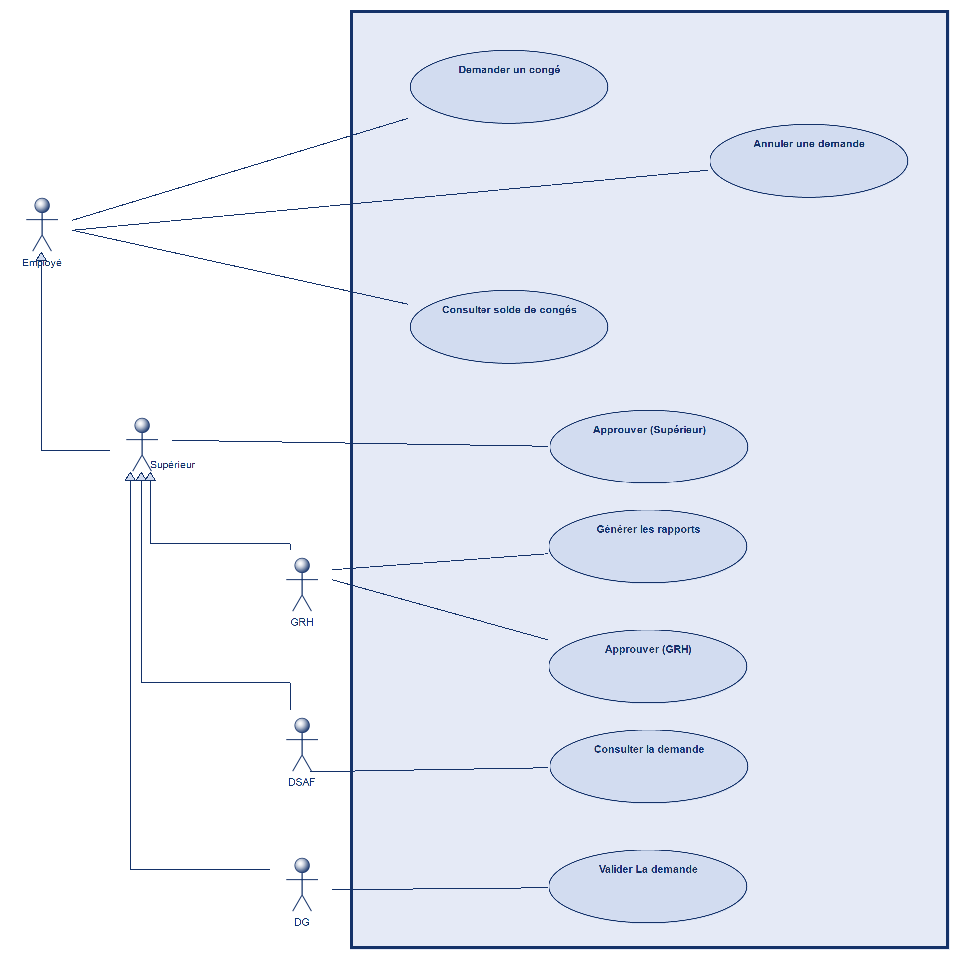
\includegraphics[width=0.8\textwidth]{images/diagrammes/use-cases/conges.png}
    \caption{Diagramme de cas d'utilisation Gestion des Congés et Absences}
    \label{fig:use_case_gestion_conges}

\end{figure}
\subsubsection{Diagramme de processus}
Le diagramme de processus modélise les étapes d'exécution de certaines fonctionnalités clés du système. Le diagramme de processus pour la gestion des congés et des absences est le suivant :
\begin{figure}[H]
    \centering
    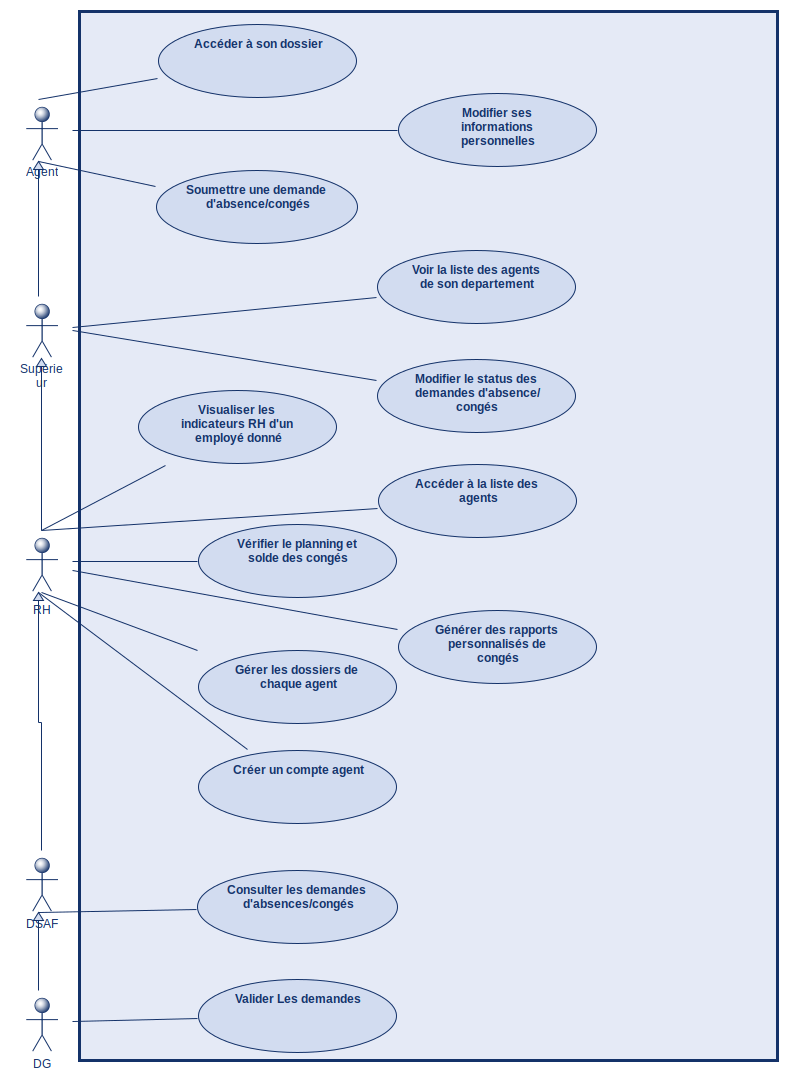
\includegraphics[width=0.8\textwidth]{images/diagrammes/flowcharts/conges.png}
    \caption{Diagramme de processus Gestion des Congés et Absences}
    \label{fig:flow_gestion_conges}
\end{figure}

\subsection{Gestion des dossiers}
\subsubsection{Description de la fonctionnalité}
La gestion des dossiers permet aux employés de consulter leur dossier personnel en ligne, de télécharger des bulletins de paie, et de demander des documents administratifs.
\subsubsection{Description des cas d'utilisation}
\begin{itemize}
    \item \textbf{Consultation du dossier personnel :} L'employé peut consulter son dossier personnel en ligne, contenant ses congés, absences, formations, et évaluations.
    \item \textbf{Téléchargement des bulletins de paie :} L'employé peut télécharger ses bulletins de paie depuis l'application.
    \item \textbf{Demande de documents administratifs :} L'employé peut demander des documents administratifs en ligne, tels que des attestations de travail, des certificats de travail.
\end{itemize}
\subsubsection{Diagramme de cas d'utilisation}
\begin{figure}[H]
    \centering
    \includegraphics[width=0.8\textwidth]{images/diagrammes/use-cases/dossiers.png}
    \caption{Diagramme de cas d'utilisation Gestion des dossiers}
    \label{fig:use_case_gestion_dossiers}
\end{figure}
\subsubsection{Diagramme de processus}
Le diagramme de processus pour la gestion des dossiers est le suivant :
\begin{figure}[H]
    \centering
    \includegraphics[width=0.8\textwidth]{images/diagrammes/flowcharts/dossiers.png}
    \caption{Diagramme de processus Gestion des dossiers}
    \label{fig:flow_gestion_dossiers}
\end{figure}
\subsection{Publication des notes et informations}
\subsubsection{Description de la fonctionnalité}
La publication des notes et des informations permet au GRH de publier des notes, des informations, et des documents RH pour les employés, avec des alertes et des notifications pour les rappeler des échéances.
\subsubsection{Description des cas d'utilisation}   
\begin{itemize}
    \item \textbf{Publication des notes et informations :} Le GRH peut publier des notes, des informations, et des documents RH pour les employés.
    \item \textbf{Alertes et notifications :} Les employés reçoivent des alertes et des notifications pour les rappeler des échéances, des actions sur les demandes.
\end{itemize}
\subsubsection{Diagramme de cas d'utilisation}
\begin{figure}[H]
    \centering
    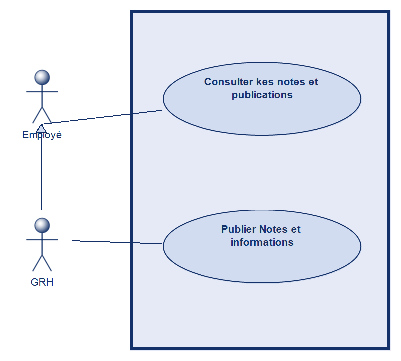
\includegraphics[width=0.8\textwidth]{images/diagrammes/use-cases/note.png}
    \caption{Diagramme de cas d'utilisation Publication des notes et informations}
    \label{fig:use_case_publication}
\end{figure}
\subsubsection{Diagramme de processus}
Le diagramme de processus pour la publication des notes et des informations est le suivant :
\begin{figure}[H]
    \centering
    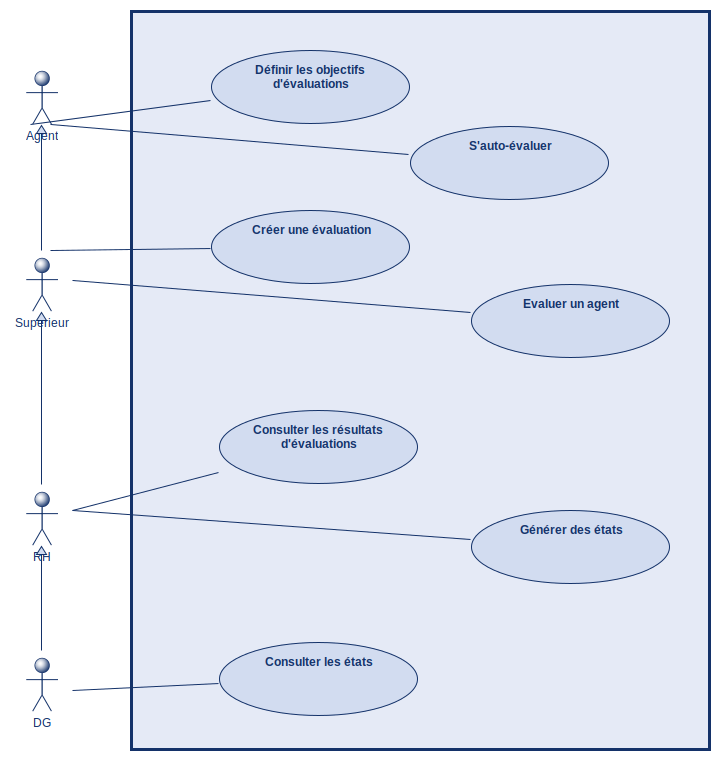
\includegraphics[width=0.8\textwidth]{images/diagrammes/flowcharts/note.png}
    \caption{Diagramme de processus Publication des notes et informations}
    \label{fig:flow_publication}
\end{figure}

\section{Conclusion}
Ce cahier des charges définit les fonctionnalités et les exigences techniques d'un logiciel de gestion RH performant et sécurisé pour l'ARCOP. Le logiciel, nommé \textbf{OptiHR}, répondra aux besoins spécifiques du GRH et des employés, en facilitant la gestion des congés, des formations, et des évaluations, d'éditer les bulletins de paie tout en étant évolutif et intégrable aux systèmes existants. La prochaine étape consistera à concevoir l'architecture du système et à élaborer les diagrammes UML pour modéliser les interactions entre les différents modules.
\clearpage

%-------------------------------------------------------------------+
\chapter{Conception}
\clearpage

\section{Introduction}
La phase de conception est une étape essentielle du cycle de développement d'un projet. Elle permet de définir l'architecture globale, les composants principaux et les interactions entre les modules du système. Cette étape inclut également l'identification des acteurs du système, c'est-à-dire les utilisateurs et les entités interagissant avec celui-ci, afin d'adapter les fonctionnalités aux besoins réels. Une conception rigoureuse garantit une meilleure organisation du projet et facilite sa mise en œuvre ainsi que sa maintenance.

\section{Objectifs}
Les objectifs de la phase de conception sont les suivants :
\begin{itemize}
    \item Identifier et structurer les différents composants du système.
    \item Définir l'architecture logicielle en fonction des besoins du projet.
    \item Spécifier les interactions entre les modules pour assurer une cohérence globale.
    \item Concevoir les diagrammes UML, y compris les diagrammes de classes et de processus, afin de modéliser clairement la structure et le fonctionnement du système.
    \item Optimiser la conception en tenant compte des performances et de l'évolutivité.
    \item Assurer la conformité aux standards et aux bonnes pratiques du développement logiciel.
\end{itemize}


\section{Modélisation et diagrammes}

\subsection{Modélisation des données}
La modélisation des données repose sur une approche relationnelle, en raison de l'utilisation de \textbf{PostgreSQL}. Elle comprend :
\begin{itemize}
    \item La définition des entités principales et de leurs relations.
    \item L'organisation des tables et la gestion des clés primaires et secondaires.
    \item L'utilisation des \textbf{migrations Laravel} pour gérer la structure de la base de données.
\end{itemize}

\subsection{Dictionnaire de données}
Le dictionnaire de données décrit en détail les attributs des entités de la base de données, y compris leurs types, leurs rôles et leurs relations. Il permet d'assurer la cohérence et la structuration correcte des informations stockées.

\renewcommand{\arraystretch}{1.3} % Améliore l'espacement du tableau

\begin{longtable}{|p{3.5cm}|p{3.5cm}|p{3cm}|p{5cm}|}
    \hline
    \textbf{Nom de la table} & \textbf{Nom de l'attribut} & \textbf{Type de données} & \textbf{Description} \\
    \hline
    \endfirsthead

    \hline
    \textbf{Nom de la table} & \textbf{Nom de l'attribut} & \textbf{Type de données} & \textbf{Description} \\
    \hline
    \endhead

    % User
    \hline
    User & username & string & Nom d'utilisateur \\
    \hline
    User & password & string & Mot de passe \\
    \hline
    User & active & string & Statut actif/inactif \\
    \hline
    
    % Role
    Role & name & string & Nom du rôle \\
    \hline
    
    % Permission
    Permission & name & string & Nom de la permission \\
    \hline

    % Employee
    Employee & first\_name & string & Prénom de l'employé \\
    \hline
    Employee & last\_name & string & Nom de famille de l'employé \\
    \hline
    Employee & phone\_number & string & Numéro de téléphone \\
    \hline
    Employee & email & string & Adresse email \\
    \hline
    Employee & address1 & string & Adresse principale \\
    \hline
    Employee & address2 & string & Adresse secondaire \\
    \hline
    Employee & city & string & Ville \\
    \hline
    Employee & country & string & Pays \\
    \hline
    Employee & state & string & Région ou état \\
    \hline
    Employee & bank\_name & string & Nom de la banque \\
    \hline
    Employee & rib & string & Relevé d'identité bancaire \\
    \hline

    % Department
    Department & name & string & Nom du département \\
    \hline

    % File
    File & name & string & Nom du fichier \\
    \hline
    File & url & string & URL du fichier \\
    \hline
    File & mime\_type & string & Type MIME \\
    \hline
    File & path & string & Chemin d'accès \\
    \hline
    File & upload\_date & string & Date d'upload \\
    \hline

    % Duty
    Duty & duration & string & Durée de la mission \\
    \hline
    Duty & begin\_date & string & Date de début \\
    \hline
    Duty & type & string & Type de mission \\
    \hline
    Duty & etat & string & État de la mission \\
    \hline

    % Job
    Job & title & string & Intitulé du poste \\
    \hline

    % Absence
    Absence & day\_requested & string & Jour demandé \\
    \hline
    Absence & start\_date & string & Date de début \\
    \hline
    Absence & end\_date & string & Date de fin \\
    \hline
    Absence & address & string & Adresse \\
    \hline
    Absence & date\_of\_application & string & Date de la demande \\
    \hline
    Absence & status & string & Statut de l'absence \\
    \hline
    Absence & date\_of\_approval & string & Date d'approbation \\
    \hline
    Absence & type\_of\_absence & string & Type d'absence \\
    \hline
    Absence & reasons & string & Raisons de l'absence \\
    \hline
    Absence & proof & string & Justificatif \\
    \hline
    Absence & comment & string & Commentaire \\
    \hline

\end{longtable}




\subsection{Diagramme de classes}
Le diagramme de classes permet de représenter les différentes entités du système et leurs relations. Il offre une vision claire de la structure et facilite la compréhension des interactions entre les objets.

\begin{figure}[H]
    \centering
    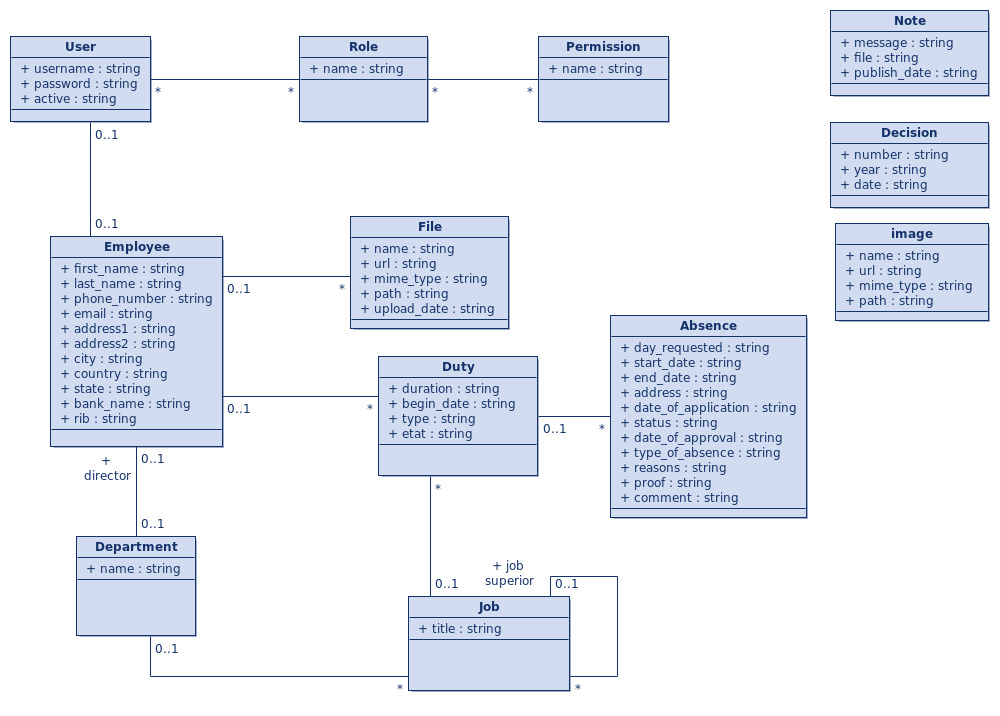
\includegraphics[width=0.8\textwidth]{images/diagrammes/class/diagramme.jpeg}
    \caption{Diagramme de classe - Gestion du projet OptiHR}
    \label{fig:class_diagramm_optiRH}
\end{figure}

\section{Description des entités et relations}

Le diagramme de classes représente un système de gestion des employés et de leurs activités professionnelles. Voici une description des entités principales et de leurs relations :

\subsection{Entités principales}

\subsubsection{User (Utilisateur)}
\textbf{Attributs} :
\begin{itemize}
    \item username
    \item password
    \item active
\end{itemize}
\textbf{Relations} : Un utilisateur est associé à un employé.

\subsubsection{Employee (Employé)}
\textbf{Attributs} :
\begin{itemize}
    \item first\_name
    \item last\_name
    \item phone\_number
    \item email
    \item address1
    \item address2
    \item city
    \item country
    \item state
    \item bank\_name
    \item rib
\end{itemize}
\textbf{Relations} :
\begin{itemize}
    \item Un employé peut être un directeur d'un département.
    \item Un employé appartient à un seul département.
    \item Un employé peut avoir plusieurs fichiers associés.
    \item Un employé peut être lié à plusieurs absences.
\end{itemize}

\subsubsection{Department (Département)}
\textbf{Attributs} :
\begin{itemize}
    \item name
\end{itemize}
\textbf{Relations} :
\begin{itemize}
    \item Un département peut avoir un seul directeur (Employee).
    \item Un département peut contenir plusieurs employés.
\end{itemize}

\subsubsection{Role (Rôle)}
\textbf{Attributs} :
\begin{itemize}
    \item name
\end{itemize}
\textbf{Relations} : Un utilisateur peut avoir plusieurs rôles.

\subsubsection{Permission (Permission)}
\textbf{Attributs} :
\begin{itemize}
    \item name
\end{itemize}
\textbf{Relations} : Un rôle peut avoir plusieurs permissions.

\subsubsection{File (Fichier)}
\textbf{Attributs} :
\begin{itemize}
    \item name
    \item url
    \item mime\_type
    \item path
    \item upload\_date
\end{itemize}
\textbf{Relations} : Un employé peut avoir plusieurs fichiers.

\subsubsection{Duty (Tâche/Mission)}
\textbf{Attributs} :
\begin{itemize}
    \item duration
    \item begin\_date
    \item type
    \item etat
\end{itemize}
\textbf{Relations} : Un employé peut avoir plusieurs tâches.

\subsubsection{Job (Poste)}
\textbf{Attributs} :
\begin{itemize}
    \item title
\end{itemize}
\textbf{Relations} : Un employé peut avoir un seul poste.

\subsubsection{Absence (Absence)}
\textbf{Attributs} :
\begin{itemize}
    \item day\_requested
    \item start\_date
    \item end\_date
    \item address
    \item date\_of\_application
    \item status
    \item date\_of\_approval
    \item type\_of\_absence
    \item reasons
    \item proof
    \item comment
\end{itemize}
\textbf{Relations} : Un employé peut avoir plusieurs absences.

\subsubsection{Note (Note)}
\textbf{Attributs} :
\begin{itemize}
    \item message
    \item file
    \item publish\_date
\end{itemize}

\subsubsection{Decision (Décision)}
\textbf{Attributs} :
\begin{itemize}
    \item number
    \item year
    \item date
\end{itemize}

\subsubsection{Image (Image)}
\textbf{Attributs} :
\begin{itemize}
    \item name
    \item url
    \item mime\_type
    \item path
\end{itemize}














\section{Technologies et outils}
Les outils et technologies suivants ont été utilisés pour la conception du projet \textbf{OptiHR}. Chaque outil est accompagné d'une image et d'une description détaillée.

\vspace{1cm} % Ajoute un espace vertical

\renewcommand{\arraystretch}{1.5} % Espacement entre les lignes du tableau

\begin{center}
\begin{tabular}{|m{4cm}|m{10cm}|}
    \hline
    \textbf{Technologie} & \textbf{Description} \\
    \hline
    
    
\includegraphics[width=3cm]{images/logo/uml.png} & \textbf{UML} : Utilisé pour la modélisation des systèmes et la conception des structures du projet. Il permet de représenter graphiquement les différentes interactions et processus du système. \\
    \hline
    
    
\includegraphics[width=3cm]{images/logo/modelio.png} & \textbf{Modelio} : Outil de modélisation UML permettant de créer des diagrammes tels que les diagrammes de classes, de séquence et d'activités. \\
    \hline
 
  
\end{tabular}
\end{center}

\section{Conclusion}
La phase de conception pose les bases essentielles du projet en structurant l'architecture et en précisant les technologies et les modèles de données adoptés. Une conception rigoureuse garantit un développement fluide et efficace, tout en assurant la maintenance et l'évolutivité du système sur le long terme.

\clearpage

%-------------------------------------------------------------------+
\chapter{Réalisation}
\clearpage
\section{Introduction}
Cette section détaille la mise en œuvre technique du projet \textbf{OptiHR}. Après la phase de conception, il est essentiel de transformer les modèles et les spécifications en un système fonctionnel. Cette phase couvre l'implémentation des différentes fonctionnalités, les choix technologiques adoptés ainsi que l'organisation du code et du développement.

\section{Choix technologiques}
Pour assurer la performance, la maintenabilité et l’évolutivité du système, les technologies suivantes ont été utilisées :
\begin{itemize}
    \item \textbf{Backend} : Laravel, un framework PHP robuste facilitant le développement d’applications web grâce à son architecture MVC.
    \item \textbf{Base de données} : PostgreSQL, un SGBD relationnel offrant une gestion avancée des données.
    \item \textbf{Frontend} : Blade, le moteur de template de Laravel, permettant de structurer l'affichage des interfaces utilisateur.
    \item \textbf{Versioning} : Git, avec un workflow basé sur GitHub pour la gestion collaborative du code source.
    \item \textbf{API} : Des endpoints RESTful ont été développés pour permettre la communication entre le frontend et le backend.
\end{itemize}

\section{Architecture et organisation du projet}
Le projet est organisé selon une architecture MVC (Modèle-Vue-Contrôleur) qui permet de séparer les différentes responsabilités et d'améliorer la maintenabilité du code :
\begin{itemize}
    \item \textbf{Modèle} : Définit les entités de la base de données et leur relation.
    \item \textbf{Vue} : Gère l’affichage des pages à l’aide de Blade.
    \item \textbf{Contrôleur} : Traite les requêtes et interagit avec les modèles pour retourner les bonnes réponses.
\end{itemize}

Le projet est structuré comme suit :
\begin{itemize}
    \item \textbf{/app} : Contient les modèles et les contrôleurs.
    \item \textbf{/resources/views} : Contient les vues Blade.
    \item \textbf{/routes} : Définit les routes du projet (web et API).
    \item \textbf{/database/migrations} : Contient les fichiers de migration pour la gestion de la base de données.
\end{itemize}

\section{Implémentation des fonctionnalités}
Les principales fonctionnalités implémentées sont :
\subsection{Gestion des utilisateurs}
\begin{itemize}
    \item Authentification des utilisateurs (inscription, connexion, déconnexion).
    \item Gestion des rôles et permissions.
\end{itemize}

\subsection{Gestion des employés}
\begin{itemize}
    \item Création, modification et suppression des employés.
    \item Attribution d’un poste et d’un département à chaque employé.
\end{itemize}

\subsection{Gestion des absences}
\begin{itemize}
    \item Saisie et validation des demandes d'absence.
    \item Suivi des statuts des absences.
\end{itemize}

\subsection{Gestion des fichiers et documents}
\begin{itemize}
    \item Upload et gestion des fichiers associés aux employés.
    \item Stockage sécurisé des documents dans le serveur.
\end{itemize}

\section{Tests et validation}
Pour garantir la fiabilité du système, plusieurs tests ont été réalisés :
\begin{itemize}
    \item \textbf{Tests unitaires} : Vérification des fonctionnalités des modèles et des contrôleurs.
    \item \textbf{Tests fonctionnels} : Vérification du bon fonctionnement des fonctionnalités majeures.
    \item \textbf{Tests d'intégration} : Vérification des interactions entre les différents modules.
    \item \textbf{Tests utilisateurs} : Validation des fonctionnalités par des tests en conditions réelles.
\end{itemize}

\section{Déploiement}
Le déploiement du projet a été effectué selon les étapes suivantes :
\begin{itemize}
    \item Configuration du serveur et installation des dépendances.
    \item Migration de la base de données et initialisation des données.
    \item Déploiement sur un serveur web avec Nginx et Laravel.
    \item Configuration des sauvegardes et de la sécurité.
\end{itemize}

\section{Conclusion}
La phase de réalisation a permis d'implémenter les fonctionnalités prévues et d'assurer la mise en production d'un système fonctionnel et performant. Grâce à une approche modulaire et une gestion rigoureuse du code, le projet OptiHR est désormais prêt à être utilisé par les utilisateurs finaux.
\clearpage

%-------------------------------------------------------------------+
\chapter{Bilan}

%-------------------------------------------------------------------+
\chapter{Conclusion Générale}
\clearpage

\end{document}